\documentclass[12pt,a4paper]{book}
\usepackage[latin1]{inputenc}
%\usepackage{creativecommons}
\usepackage{xmpincl}
\usepackage{lipsum}
\usepackage{url}
\usepackage{amsmath}
\usepackage{amsfonts}
\usepackage{amssymb}
\usepackage{graphicx}
\usepackage{multicol}
\usepackage[normalem]{ulem} % needed by strike
\usepackage[urlcolor=blue,colorlinks=true,citecolor=blue,linkcolor=black]{hyperref}
\usepackage{makeidx}
\usepackage{color}
\usepackage{xmpincl}
\makeindex
\setcounter{tocdepth}{1}
\author{Paul Sutton}
\begin{document}

\begin{figure}
\centering
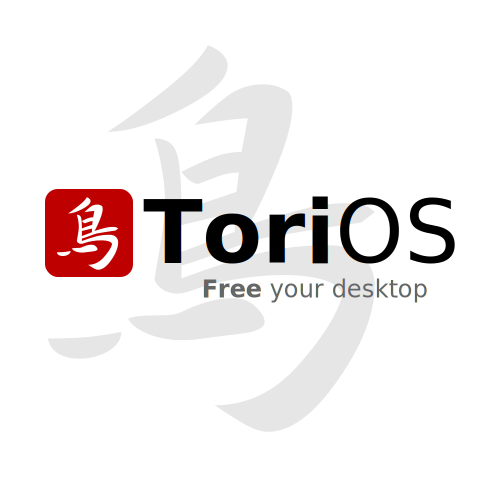
\includegraphics[width=0.7\linewidth]{./FinalLogo}

\begin{center}
{\Huge ToriOS Testing Manual}
\end{center}

\end{figure}

\tableofcontents
\index{Table of Contents}

\chapter{Introduction}
This manual is intended to act as a guide to help people test ToriOS and give brief overviews in to the different ways that ToriOS can be tested. 

\chapter{Virtual-Box}
\index{Virtualbox}
Text added to make Contents work
\textbf{Part 1 : set up virtual box - GNU / Linux}
To set install Virtual box on Ubuntu you should run the following \\

\begin{itemize}
\item{sudo apt-get install virtualbox-qt}
\item{sudo apt-get install virtualbox-dkms}
\end{itemize} 

After this you need to set up a virtual machine so that the MiniISO can be installed to this.   It is ASSUMED you know how to do this.  However you DO need to enable networking:\\ \\
\includegraphics[width=0.7\linewidth]{screen-shots/virtualbox-network} \\

You may also want to check to see if PAE has been enabled as toriOS is designed for NON PAE systems.\\
\includegraphics[width=0.7\linewidth]{screen-shots/Virtualbox-enablePAE}


Once done you can run virtual box from the menu.

Compomemts such as USB amd sharing files with the host system are NOT supported unless using virtualbox extensions.  \\



\chapter{Obtaining the Ubuntu Mini ISO}

This step covers what is needed to convert a ubuntu 12.04 mini ISO to use the ToriOS desktop environment and related system components.\\ \\
\textbf{
Step 1:} Install ToriOS into the virtual machine created earlier. 

Download the iso file from the website below \\

http://archive.ubuntu.com/ubuntu/dists/precise-updates/main/installer-i386/current/images/

netboot directory then nonPAE

file mini.iso

You will also need to download the md5sum checksum and verify the download. 

\chapter{Convert mini ISO to ToriOS}

Once you have downloaded and installed the Mini ISO you should be logged in as a default user,  and this user should be a member of the sudo-ers list so you can run sudo (as in run a command as root) as that user. \\
in which case you can wget the shell script and run that to convert to ToriOS\\

Download shell script
wget https://raw.githubusercontent.com/Israel-/torios-from-mini/master/torios-precise-x86.sh

set to execute permissions

chmod +x torios-precise-x86.sh


You can use wget -c for this
\chapter{Install - blank HDD}
Text added to make Contents work

\chapter{Install - Multi-Boot} 




\printindex

\end{document}